\documentclass[11pt,english]{article}
\usepackage[T1]{fontenc}
\usepackage{babel}
\usepackage[margin=0.8 in]{geometry}
\usepackage{caption}
\usepackage{subfig}
\usepackage{longtable}
\usepackage{natbib}
\linespread{1.15}
\usepackage{tikz}
\usepackage{setspace}
\usepackage{multirow}
\usepackage{multicol}
\usepackage{csquotes}
% ------
% Fonts and typesetting settings


%\usepackage[sc]{mathpazo}
\usepackage{titling}									
\usepackage{float}
\usepackage{pdflscape}
\usepackage[toc]{appendix}
\renewcommand{\appendixtocname}{Appendices}
%\renewcommand{\appendixsection}{\normalfont\bfseries}
\usepackage{amsmath, amsthm, amsfonts}


\newcommand{\subtitle}[1]{%
  \posttitle{%
    \par\end{center}
    \begin{center}\large#1\end{center}
    \vskip0.5em}%
}

\usepackage{booktabs}												
\usepackage{natbib}                                                 
\usepackage{graphics,epsfig}						
% -----
% ------



% Maketitle metadata
\author{
Natalia Serna
   }
 \title{Problem set 1}

\date{}
%%%%%%%%%%%%%%%%%%%%%%%%
\begin{document}

\maketitle

\section{Problem 1}

\begin{enumerate}
\item Given the information in the problem, the price elasticity of demand is:
\textcolor{blue}{\begin{align}
|\varepsilon|=\left|\frac{\partial Q}{\partial P}\frac{P}{Q}\right|=\left(\frac{1}{a_{1}}\right)\left(\frac{a_{0}-a_{1}Q+v}{Q}\right)\nonumber
\end{align}}
Differentiating this expression with respect to $v$ we get:
\begin{align}
\frac{\partial|\varepsilon|}{\partial v}=\frac{1}{a_{1}Q}\geq0\nonumber
\end{align}
This suggests the price elasticity of demand increases as the maximum willingness to pay increases. This can also be interpreted in terms of the dispersion of the willingness to pay: the higher the dispersion, the more sensitive is the quantity demanded to changes in price.

Differentiating with respect to $Q$ we get:
\begin{align}
\frac{\partial|\varepsilon|}{\partial v}&=\frac{-a_{1}^{2}Q-a_{0}a_{1}+a_{1}^{2}Q-a_{1}v}{a_{1}^{2}Q}\nonumber\\
&=\frac{-a_{0}a_{1}-a_{1}v}{a_{1}^{2}Q}\nonumber\\
&\leq0 \iff v\geq -a_{0}\nonumber
\end{align}

In this case, under the assumption that $v+a_{0}\geq0$, the price elasticity of demand decreases as total quantity increases. Intuitively, as total quantity demanded increases we are moving to the right along the demand curve, reaching a portion where prices are small relative to quantities.

\item For a fixed $N$, the problem of firm $i$ is
\[
Max_{q_{i}} \ \ (a_{0}-a_{1}(q_{i}+Q_{-i})+v-b_{0}-\eta)q_{i}-F
\]
Taking the first order condition, we get:
\[
a_{0}-2a_{1}q_{i}-a_{1}Q_{-i}+v-b_{0}-\eta=0
\]
Because the best response functions for each firm are symmetric, we can focus on the symmetric equilibrium where $q_{i}=q$, $\forall i$. Then, solving for $q$ from the FOC:

\[
\textcolor{blue}{q=\frac{a_{0}+v-b_{0}-\eta}{a_{1}(N+1)}}
\]

So total quantity is:
\[
\textcolor{blue}{Q=N\left(\frac{a_{0}+v-b_{0}-\eta}{a_{1}(N+1)}\right)}
\]

Price is:
\[
\textcolor{blue}{P=\frac{a_{0}+v+N(b_{0}+\eta)}{N+1}}
\]

And equilibrium profits are:
\[
\textcolor{blue}{\pi=\frac{1}{a_{1}}\left(\frac{a_{0}+v-b_{0}-\eta}{N+1}\right)^{2}-F}
\]

\item Using the zero profit condition and the equilibrium profits derived above, the optimal number of firms is given by:
\begin{align}
\pi=0\iff &\left(\frac{a_{0}+v-b_{0}-\eta}{N+1}\right)^{2}=a_{1}F\nonumber\\
\iff &\frac{a_{0}+v-b_{0}-\eta}{N+1}=\sqrt{a_{1}F}\nonumber\\
\iff&\textcolor{blue}{N=\frac{a_{0}+v-b_{0}-\eta}{\sqrt{a_{1}F}}-1}\nonumber
\end{align}

\item With our results for the equilibrium price, quantity, and number of firms, the Lerner index is:
\begin{align}
\mathcal{L}&=\frac{P-mc}{P}=\frac{a_{0}+v-b_{0}-\eta}{a_{0}+v-N(b_{0}+\eta)}\iff \textcolor{blue}{\mathcal{L}=\frac{\sqrt{a_{1}F}}{\sqrt{a_{1}F}+b_{0}+\eta}}\nonumber
\end{align}

The HHI by definition is:
\begin{align}
\mathcal{HHI}&=\frac{1}{N}\iff\textcolor{blue}{\mathcal{HHI}=\frac{\sqrt{a_{1}F}}{a_{0}+v-b_{0}-\eta-\sqrt{a_{1}F}}}\nonumber
\end{align}

And the elasticity of demand is:
\begin{align}
\textcolor{blue}{|\varepsilon|=\frac{\sqrt{a_{1}F}+b_{0}+\eta}{a_{0}+v-b_{0}-\eta-\sqrt{a_{1}F}}}\nonumber
\end{align}

\item Differentiating the expression for the elasticity of demand with respect to $v$ we get:

\begin{align}
\frac{\partial \varepsilon}{\partial v}=-\frac{\sqrt{a_{1}F}+b_{0}+\eta}{(a_{0}+v-b_{0}-\eta-\sqrt{a_{1}F})^{2}}\leq0\nonumber
\end{align}

Notice that this relation is of the opposite sign compared to the situation where the market structure is exogenous. In the case of endogenous market structure we find that the price elasticity of demand decreases as the maximum willingness to pay increases. This suggests that the indirect effect that an increase in the willingness to pay has on the number firms dominates the direct effect of a movement outwards of the demand curve. As willingness to pay rises, the number of firms increases, with each of them producing $\sqrt{F/a_{1}}$, so equilibrium quantity goes up and we move to the right along the demand curve past the point of unit elasticity.


Differentiating the elasticity with respect to $\eta$ we get:

\begin{align}
\frac{\partial \varepsilon}{\partial \eta}=\frac{a_{0}+v}{(a_{0}+v-b_{0}-\eta-\sqrt{a_{1}F})^{2}}\geq0\nonumber
\end{align}

Which means that as the marginal cost increases, the elasticity of demand increases as well. The intuition is that as marginal cost rises, each firm is going to decrease production, so total quantity falls and we move to the left along the demand curve to the portion where it is more elastic.

Differentiating the elasticity with respect to $F$ we get:

\begin{align}
\frac{\partial \varepsilon}{\partial F}=\frac{(a_{0}+v)\sqrt{a_{1}}}{2\sqrt{F}(a_{0}+v-b_{0}-\eta-\sqrt{a_{1}F})^{2}}\geq0\nonumber
\end{align}

In this case, although fixed costs are sunk when firms are deciding on their level of production, a higher fixed cost of entry reduces the potential number of firms in the market which shrinks total quantity and generate the same movement to the left along the demand curve as before.

In terms of the Lerner index, define its log scale as:
\begin{align}
ln(\mathcal{L})=0.5ln(a_{1})+0.5ln(F)-ln(\sqrt{a_{1}F}+b_{0}+\eta)\nonumber
\end{align}

Differentiating this expression with respect to F, $v$ and $\eta$ we get:
\begin{align}
\frac{\partial ln(\mathcal{L})}{\partial F}&=\frac{b_{0}+\eta}{2F(\sqrt{a_{1}F}+b_{0}+\eta)}\geq0\nonumber\\
\frac{\partial ln(\mathcal{L})}{\partial v}&=0\nonumber\\
\frac{\partial ln(\mathcal{L})}{\partial \eta}&=-\frac{1}{\sqrt{a_{1}F}+b_{0}+\eta}\leq0\nonumber
\end{align}

So these results indicate that as fixed costs increase, the percentage of markup over price increases as well when the market structure is endogenous. The reason is the following: as fixed costs increases, the potential number of firms in the market decreases, which shrinks total equilibrium quantity and therefore increases price. With regard to the maximum willingness to pay, in an exogenous market structure, the increase in willingness to pay would increase prices, but with endogenous structure this effect is counteracted by the increase in the number of firms. Also, an increase in marginal costs decreases the markup firms can charge by a larger amount than prices increase, so the Lerner index falls.

In terms of the HHI, define its log scale as:
\begin{align}
ln(\mathcal{HHI})=0.5ln(a_{1})+0.5ln(F)-ln(a_{0}+v-b_{0}-\eta-\sqrt{a_{1}F})\nonumber
\end{align}

Differentiating this expression with respect to F, $v$ and $\eta$ we get:
\begin{align}
\frac{\partial ln(\mathcal{HHI})}{\partial F}&=\frac{a_{0}+v-b_{0}-\eta}{2F(a_{0}+v-b_{0}-\eta-\sqrt{a_{1}F})}\geq0\nonumber\\
\frac{\partial ln(\mathcal{HHI})}{\partial v}&=-\frac{1}{a_{0}+v-b_{0}-\eta-\sqrt{a_{1}F}}\leq0\nonumber\\
\frac{\partial ln(\mathcal{HHI})}{\partial \eta}&=\frac{1}{a_{0}+v-b_{0}-\eta-\sqrt{a_{1}F}}\geq0\nonumber
\end{align}

These expressions show that as fixed costs increase so does the HHI, since the number of firms decrease. The HHI and the maximum willingness to pay are inversely related because higher willingness to pay attracts firms into the market. Finally, an increase in marginal costs, reduces the number of firms and hence increases the HHI.

From the partial derivatives we can see that $F$ has the same effect on the LI and the HHI but $\eta$ has a different effect on each of these.

\item If firms can collude, the objective is now:
\[
Max_{Q}\ (a_{0}-a_{1}Q+v-b_{0}-\eta)Q-NF
\]
Taking the first order condition, we get:
\[
a_{0}-2a_{1}Q+v-b_{0}-\eta=0
\]
So total quantity is:
\[
\textcolor{blue}{Q=\frac{a_{0}+v-b_{0}-\eta}{2a_{1}}}
\]
Individual quantity is:
\[
\textcolor{blue}{q=\frac{a_{0}+v-b_{0}-\eta}{2a_{1}N}}
\]
Price is:
\[
\textcolor{blue}{P=\frac{a_{0}+v+b_{0}+\eta}{2}}
\]

And equilibrium profits are:
\[
\textcolor{blue}{\pi_{i}=\frac{1}{4a_{1}N}(a_{0}+v-b_{0}-\eta)^{2}-F}\ \ \forall i
\]
Using the zero profit condition to solve for the number of firms we have:
\begin{align}
\pi=0\iff &\textcolor{blue}{N=\frac{(a_{0}+v-b_{0}-\eta)^{2}}{4a_{1}F}}\nonumber
\end{align}

In this case the Lerner index, HHI, and elasticity of demand are:

\textcolor{blue}{
\begin{align}
\mathcal{L}&=\frac{a_{0}+v-b_{0}-\eta}{a_{0}+v+b_{0}+\eta}\nonumber\\
\mathcal{HHI}&=\frac{4a_{1}F}{(a_{0}+v-b_{0}-\eta)^{2}}\nonumber\\
|\varepsilon|&=\frac{a_{0}+v+b_{0}+\eta}{a_{0}+v-b_{0}-\eta}\nonumber
\end{align}}

\item Given the functional form of the demand function, the elasticity is constant along the demand curve:
\[
\textcolor{blue}{|\varepsilon|=1/c_{1}}
\]
In the Cournot game, every firm is solving the following problem
\[
Max_{q_{i}}\ \left(\frac{exp(c_{0}+\xi)}{(q_{i}+Q_{-i})^{c_{1}}} -b_{0}-\eta\right)q_{i}-F
\]
Taking the first order condition, we get:
\[
\frac{exp(c_{0}+\xi)((q_{i}+Q_{-i})^{c_{1}}-(q_{i}+Q_{-i})^{c_{1}-1}c_{1}q_{i})}{(q_{i}+Q_{-i})^{2c_{1}}}-b_{0}-\eta=0
\]
Since every firm has symmetric best response function, we can focus on the symmetric equilibrium where $q_{i}=q$, $\forall i$. So solving for $q$ we get:
\[
\textcolor{blue}{q=\left(\frac{(N-c_{1})exp(c_{0}+\xi)}{(b_{0}+\eta)N^{c_{1}+1}}\right)^{1/c_{1}}}
\]
Price is:
\[
\textcolor{blue}{P=\frac{(b_{0}+\eta)N}{N-c_{1}}}
\]

And Lerner index and HHI are:

\textcolor{blue}{
\begin{align}
\mathcal{L}&=\frac{c_{1}}{N}\nonumber\\
\mathcal{HHI}&=\frac{1}{N}\nonumber
\end{align}}

From these results, the first thing that arises is that the elasticity of demand, the Lerner index, and the HHI are non responsive to changes in $F$, $v$ or $\eta$ for a fixed market structure.  Under endogenous market structure we would expect in these indicators to vary with the exogenous parameters.
\end{enumerate}

\section{Problem 2}

\begin{enumerate}

\item Table \eqref{t1} shows the regressions of the Lerner index on the HHI for the case of a log-log demand and fixed market structure. On the full sample of cities an increase of 1\% in the HHI increases the Lerner index by 0.81\%. In other words, higher concentration in terms of quantity can translate in higher market power in terms of markups.  Since market structure is exogenous there aren't potential entrants even if profits are positive, this allows firms ,in general, to charge higher prices despite the fact demand is elastic given the values of the parameters ($|\varepsilon|=1.11$).

The magnitude of the coefficient on the HHI is smaller when we condition on the subsample of cities without antitrust policy (0.68\%) than when we condition on the cities with antitrust policy (1\%). This difference can also be explained by the fact that a relatively high elasticity of demand counteracts the ability of the monopoly to charge higher prices by inducing a relatively large reduction in quantity and hence market shares. 

Table \eqref{t2} shows the t-test for the hypothesis that the coefficient on the HHI is equal to 1. For the second regression on cities with antitrust policy we cannot reject the null, while in the other regressions we do. This means that under Cournot, the Lerner index and the HHI move in the same magnitude and in the same direction, while under collusion the relation is less than proportional.


% Table generated by Excel2LaTeX from sheet 'Hoja1'
\begin{table}[H]
  \centering
  \caption{SCP regression with fixed market structure and log-log demand}
    \begin{tabular}{lrrr}
    \hline
          & Without antitrust & With antitrust & Full Sample \\
    \hline
    Constant & 0.5003*** & -0.1028*** & 0.1626*** \\
        & (0.0853) & (0.0030) & (0.0592) \\
    log(HHI) & 0.6791*** & 1.0008*** & 0.8130*** \\
        & (0.0507) & (0.0018) & (0.0356) \\
        N &500 & 500& 1000\\
    \hline
    \end{tabular}%
  \label{t1}%
\end{table}

% Table generated by Excel2LaTeX from sheet 'Hoja1'
\begin{table}[H]
  \centering
  \caption{Hypothesis testing $H_{o}: ln(HHI)=1$ with fixed market structure and log-log demand}
    \begin{tabular}{lrrr}
    \hline
          & Without antitrust & With antitrust & Full Sample \\
    \hline
    t-statistic & 6.3322 & 0.4185 & 5.2484 \\
      Reject $H_{o}$    & True & False & True \\
    \hline
    \end{tabular}%
  \label{t2}%
\end{table}

\item Table \eqref{t3} shows the regression of the Lerner index on the HHI for the case of a linear demand and fixed market structure. Results differ in magnitude compared to the previous regressions. Here an increase of 1\% in the HHI, increases the Lerner index by 0.27\% using the full sample of cities. The difference between the two models is explained by the fact that with linear demand, the elasticity depends on total equilibrium quantity while in the previous case it was constant. In this case demand is relatively more elastic compared to the log-log specification. The magnitude of the effect varies depending on the subsample of cities we use because in those without antitrust policy total equilibrium quantity is less than in those with antitrust policy, so demand elasticity is greater under the first than under the second, and hence markups can be higher in the second case but not necessarily in the first one. Figure \eqref{f1} highlights this difference in elasticity between the two subsamples.

Table \eqref{t4} shows the t-test for the hypothesis that the coefficient on the HHI is equal to 1. Using the subsamples and the full sample of cities, we can reject the null. Therefore, the HHI and the Lerner index do not move proportionately in the same direction.

% Table generated by Excel2LaTeX from sheet 'Hoja1'
\begin{table}[H]
  \centering
  \caption{SCP regression with fixed market structure and linear demand}
    \begin{tabular}{lrrr}
    \hline
          & Without antitrust & With antitrust & Full Sample \\
    \hline
    Constant & -1.0959*** & -0.6029*** & -1.0334*** \\
        & (0.0082) & (0.0068) & (0.0061) \\
    log(HHI) & 0.2699*** & 0.5161*** & 0.2669*** \\
        & (0.0049) & (0.0042) & (0.0037) \\
                N & 500&500 &100\\
    \hline
    \end{tabular}%
  \label{t3}%
\end{table}

% Table generated by Excel2LaTeX from sheet 'Hoja1'
\begin{table}[H]
  \centering
  \caption{Hypothesis testing $H_{o}: ln(HHI)=1$ with fixed market structure and linear demand}
    \begin{tabular}{lrrr}
    \hline
          & Without antitrust & With antitrust & Full Sample \\
    \hline
    t-statistic & 149.46 & 116.40 & 198.61 \\
      Reject $H_{o}$    & True & True & True \\
    \hline
    \end{tabular}%
  \label{t4}%
\end{table}

\begin{figure}[H]
\center
\caption{Distribution of price-elasticity of demand with fixed market structure for cities with and without antitrust policy}
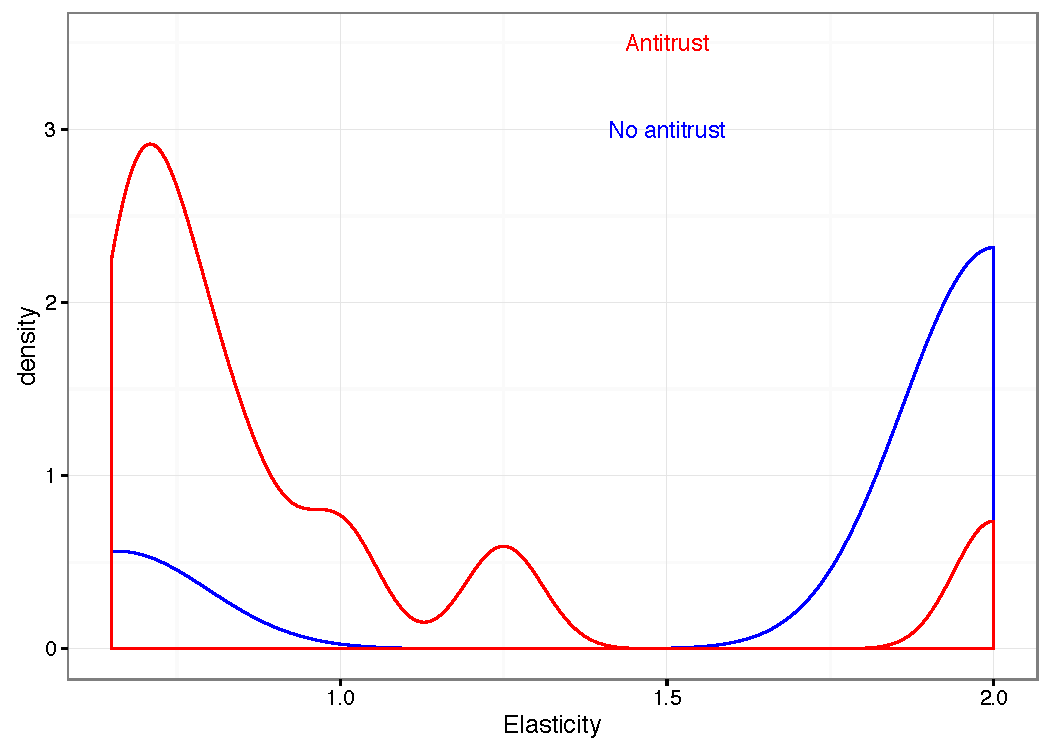
\includegraphics[width=0.5\textwidth]{elas_n_2}
\label{f1}
\end{figure}

\item From this analysis, we can see that the functional form of demand has an important impact on the conclusions we draw about collusion in markets, specially on the ability of firms to exercise market power. When we allow for the elasticity to vary along the demand curve, the ability of firms to charge higher markups is constrained by the fact they face a more elastic demand compared to the case where elasticity is constant along the demand curve. If we suspect collusion in cities 1-250, under a linear demand, we can expect the coefficient on the HHI to be even less than 0.27\%. However, under log-log demand, we would expect the coefficient to be higher.

\end{enumerate}


\section{Problem 3}


Table \eqref{t5} shows the regressions of the Lerner index on the HHI for the case of endogenous market structure and linear demand in two cases: when marginal costs are $b_{0}$ and there is variation in the maximum willingness to pay across cities (column 1) and when maximum willingness to pay is $a_{0}$ but there is variation in the marginal costs across cities (column 2). 

Volatility in the maximum willingness to pay makes it difficult to spot a pattern across cities. In particular, the finding is that the Lerner index does not respond to variations in the HHI. So compared to results in question 2, a distribution of willingness to pay that second order stochastically dominates another, allows big firms to charge higher markups. 

When there is variation in marginal costs but the maximum willingness to pay is the same across cities, the elasticity of the Lerner index with respect to the HHI is -1.12\%. Compared to the results in question 2, if a distribution of marginal costs second order stochastically dominates another one, then the aggregate effect of the HHI on the Lerner index is positive. That is, uncertainty in marginal costs translates in a lower ability of firms to charge higher markups even if they have high market shares.

We can also interpret these results in light of the elasticity of demand. Figure \eqref{f2}  shows the distribution of the elasticity for the case where $N\geq3.5$ and $N<3.5$ respectively. We can see that the elasticity is overall less dispersed when $\eta=0$ (blue)  than when $v=0$ (red). Markets where the number of firms is less than 3.5 face a more inelastic demand when there is volatility of the willingness to pay but face a more elastic demand when there is volatility of marginal costs. Therefore, in the latter case the ability to charge higher markups is restricted by the sensitivity of demand which explains the negative sign and significance on the coefficient of the HHI in the second regression. In markets where the number of firms exceeds 3.5 we can see that demand is relatively more elastic when there is volatility of the willingness to pay compared to the case where there is volatility of marginal costs. So even if demand is overall inelastic ($|\varepsilon|<1$) in these markets, the ability to charge higher markups is counteracted by competition between firms.  

% Table generated by Excel2LaTeX from sheet 'Hoja1'
\begin{table}[H]
  \centering
  \caption{SCP regression with endogenous market structure and linear demand}
    \begin{tabular}{lrr}
    \hline
          & $\eta=0$ & $v=0$ \\
    \hline
    Constant & -0.6939*** & -2.0671*** \\
        & (0.0048) & (0.0264) \\
    log(HHI) & -0.0011 & -1.1218*** \\
        & (0.0011) & (0.0205) \\
    \hline
    \end{tabular}%
  \label{t5}%
\end{table}

\begin{figure}[H]
\caption{Distribution of price-elasticity of demand conditional on N}
\subfloat[$N\geq3.5$]{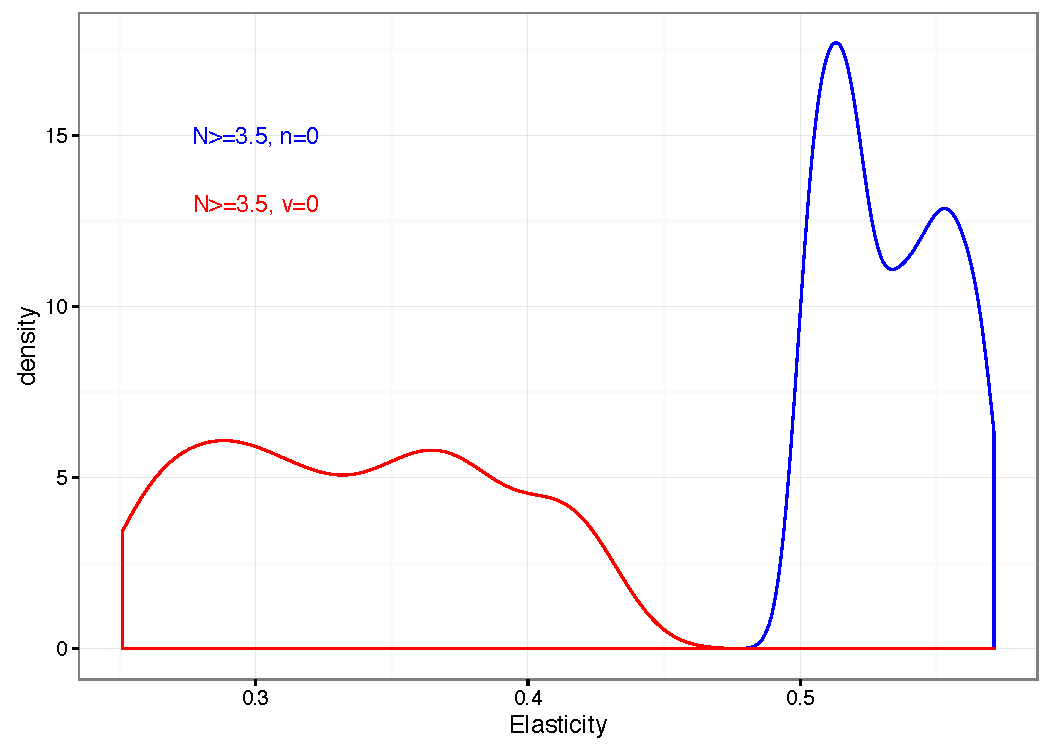
\includegraphics[width=0.5\textwidth]{elas_n_geq_3_5}}
\subfloat[$N<3$]{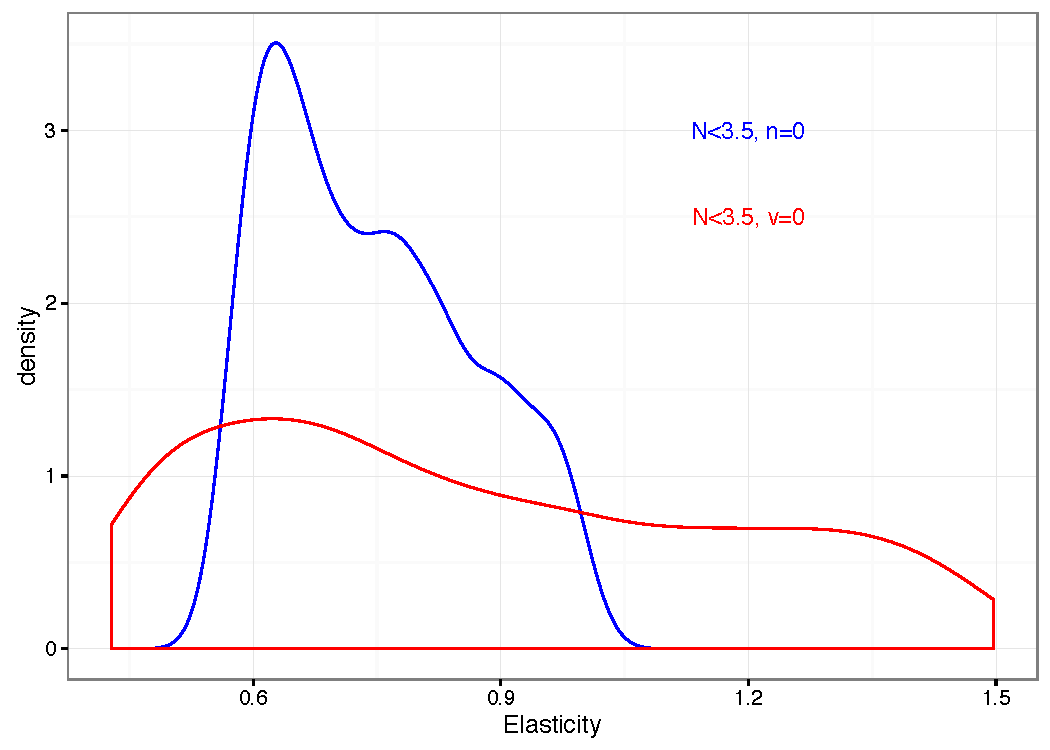
\includegraphics[width=0.5\textwidth]{elas_n_l_3_5}}
\label{f2}
\end{figure}




\end{document}